\documentclass[11pt]{article}
\usepackage[a4paper,margin=1in]{geometry}
\usepackage{graphicx}
\usepackage{caption}
\usepackage{float}
\usepackage[T1]{fontenc}
\usepackage{lmodern}
\usepackage{hyperref}

% Search for images in common locations
\graphicspath{{./}{../}{./images/}{../images/}}

\title{Zifan Si - SVM Solar Flare Classification: Report Outputs}
\author{}
\date{}

\begin{document}
\maketitle

\section*{[1/2] FEATURE EXPERIMENT (2010--2015) --- finding best feature set}
\noindent\textbf{Best feature-set COMBO on 2010--2015:} FS-I+FS-IV (TSS mean $\pm$ std $=$ 0.7773 $\pm$ 0.0395).

\begin{figure}[H]\centering
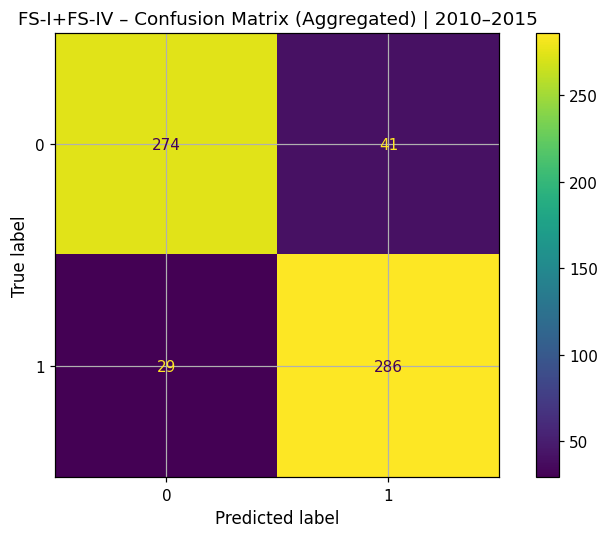
\includegraphics[width=\linewidth]{image.png}
\caption{Feature Experiment --- Plot 1}
\end{figure}

\begin{figure}[H]\centering
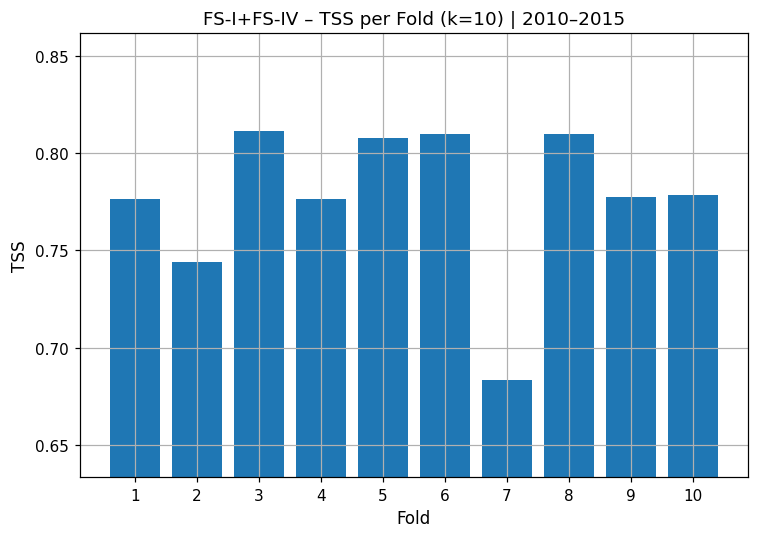
\includegraphics[width=\linewidth]{image-1.png}
\caption{Feature Experiment --- Plot 2}
\end{figure}

\begin{figure}[H]\centering
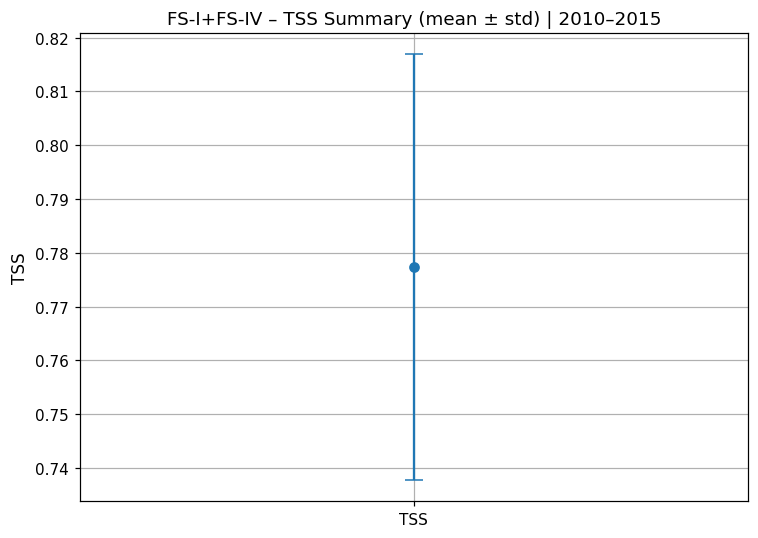
\includegraphics[width=\linewidth]{image-2.png}
\caption{Feature Experiment --- Plot 3}
\end{figure}

\section*{[2/2] DATA EXPERIMENT (2010--2015 \& 2020--2024) --- evaluating best feature set}
\noindent Using best feature-set from 2010--2015: FS-I+FS-IV

\subsection*{2010--2015}
\noindent data-2010-15 [FS-I+FS-IV]: TSS mean $\pm$ std $=$ 0.7773 $\pm$ 0.0395 (k=10).

\begin{figure}[H]\centering
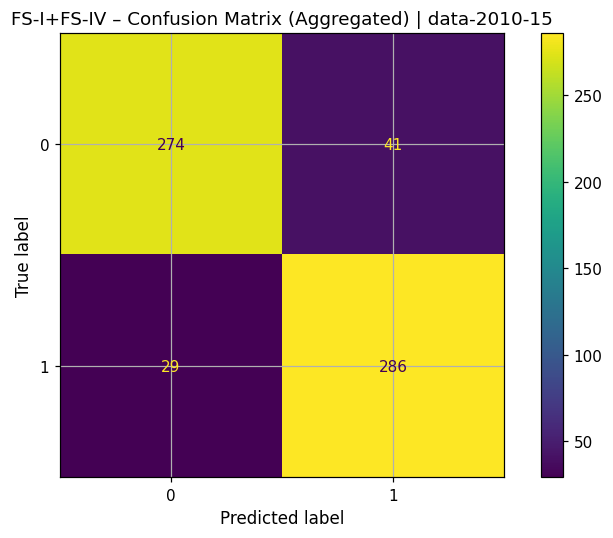
\includegraphics[width=\linewidth]{image-3.png}
\caption{2010--2015 --- Confusion Matrix}
\end{figure}

\begin{figure}[H]\centering
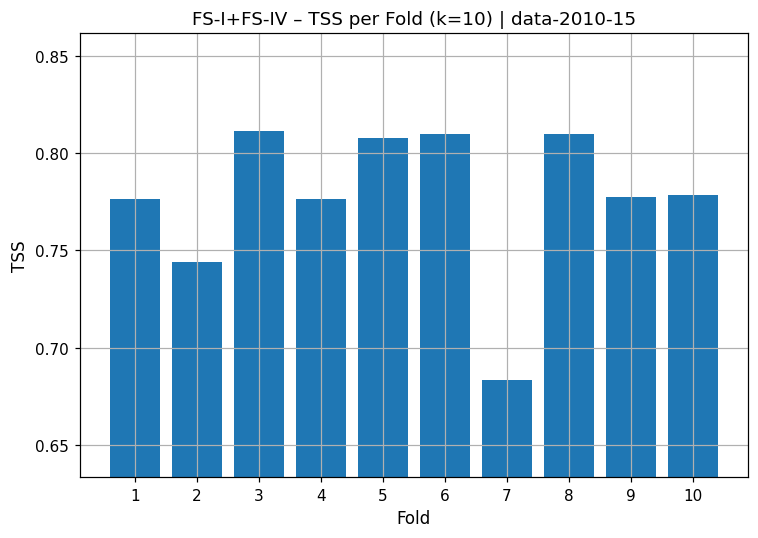
\includegraphics[width=\linewidth]{image-4.png}
\caption{2010--2015 --- TSS per Fold}
\end{figure}

\begin{figure}[H]\centering
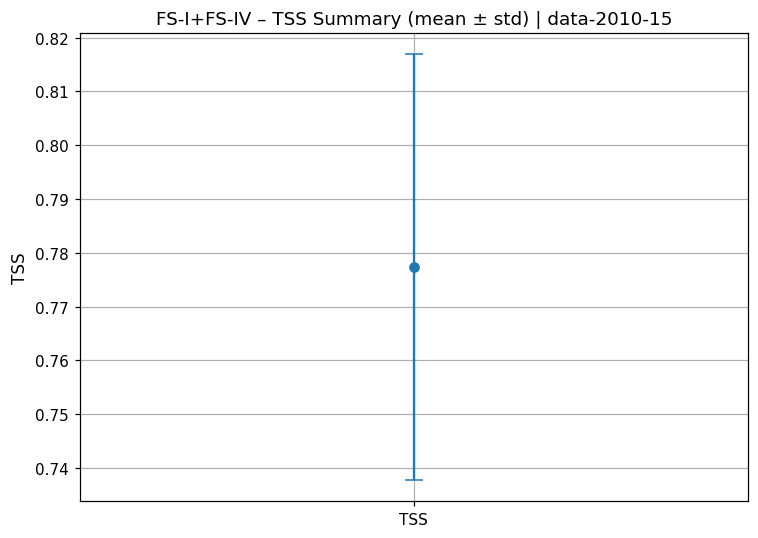
\includegraphics[width=\linewidth]{image-5.png}
\caption{2010--2015 --- TSS Summary (mean $\pm$ std)}
\end{figure}

\subsection*{2020--2024}
\noindent data-2020-24 [FS-I+FS-IV]: TSS mean $\pm$ std $=$ 0.6619 $\pm$ 0.2173 (k=10).

\begin{figure}[H]\centering
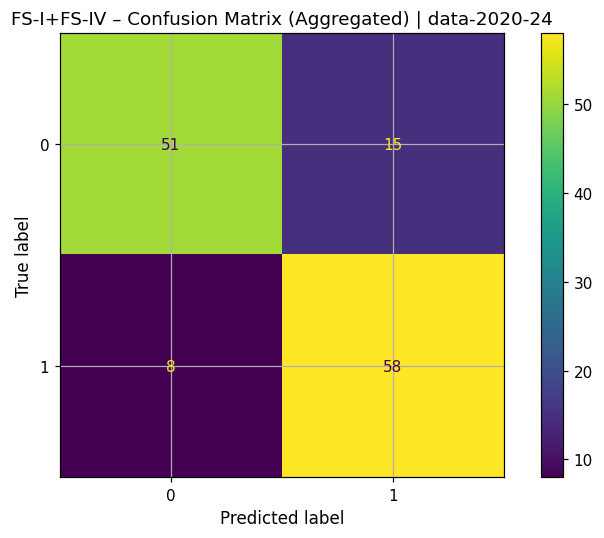
\includegraphics[width=\linewidth]{image-6.png}
\caption{2020--2024 --- Confusion Matrix}
\end{figure}

\begin{figure}[H]\centering
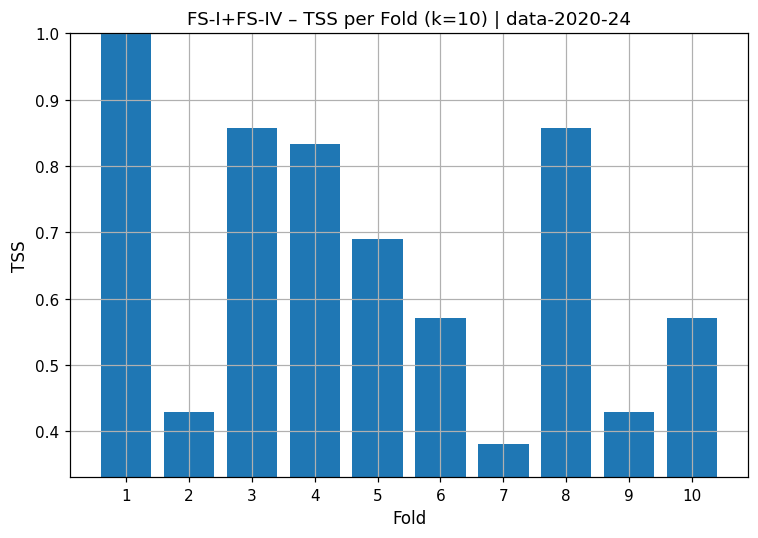
\includegraphics[width=\linewidth]{image-7.png}
\caption{2020--2024 --- TSS per Fold}
\end{figure}

\begin{figure}[H]\centering
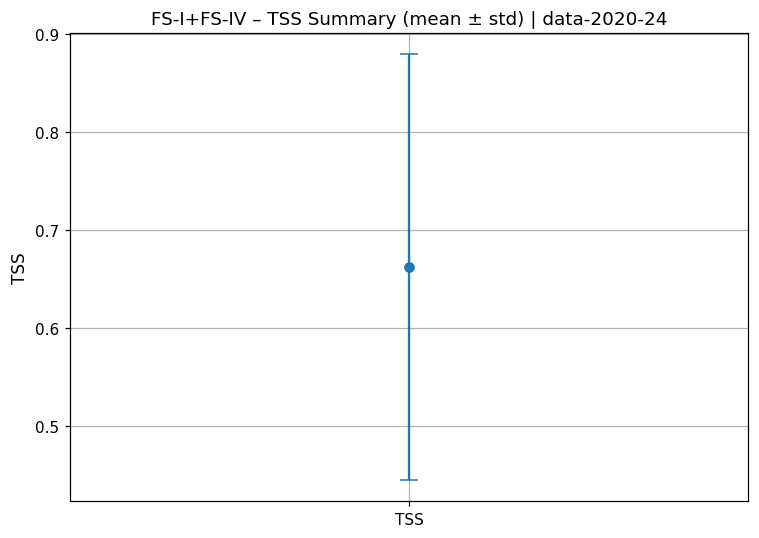
\includegraphics[width=\linewidth]{image-8.png}
\caption{2020--2024 --- TSS Summary (mean $\pm$ std)}
\end{figure}


\section*{3. Discussion / Short Answers}

\subsection*{(a) Which feature combination worked best and which was worst?}

\noindent \textbf{Best:} The combination \textbf{FS-I + FS-IV} achieved the highest overall performance 
with a True Skill Statistic (TSS) of $0.7773 \pm 0.0395$ on the 2010--2015 dataset, demonstrating that
combining the main magnetic features (FS-I) with the max–min range features (FS-IV) yields the most
discriminative representation for flare prediction. \\[6pt]

\noindent \textbf{Worst:} The \textbf{FS-III} feature set (Historical Activity only) produced the lowest
performance, with a TSS of $0.0000 \pm 0.0000$ over $k=10$ folds. This indicates that past flare
counts alone are not predictive of future events, as the model effectively performs no better than random guessing.

\begin{figure}[H]\centering
\includegraphics[width=\linewidth]{fs3.png}
\caption{FS-III --- Confusion Matrix and TSS Summary (mean $\pm$ std = $0.0000 \pm 0.0000$).}
\end{figure}

\subsection*{(b) Does adding additional feature sets improve TSS?}
\noindent Yes. Combining FS-I (main features) with FS-IV (max–min features) improved TSS by incorporating both magnitude and range information, enhancing discrimination between flare and non-flare regions.


\subsection*{(c) Which dataset led to a better TSS and why?}
\noindent The 2010–2015 dataset outperformed the 2020–2024 dataset (TSS $0.777$ vs.\ $0.662$). This difference likely stems from greater data consistency, lower measurement noise, and more balanced event representation in the 2010–2015 dataset.


\end{document}
